%! TEX program = pdflatex

\documentclass[oneside,solution]{seu-ml-assign}

\title{Assignment}
\author{Xie xing}
\studentID{58122204}
\instructor{Xu-Ying Liu}
\date{\today}
\duedate{June 12, 2024}
\assignno{5}
\semester{SEU --- 2024 Spring}
\mainproblem{Ensemble, Clustering \& Feature Selection}

\begin{document}

\maketitle

% \startsolution[print]
%第一题SVM
\problem{Bagging, Random Forest \& Feature Selection, Short Answer }


\subsection{(1) Computational Cost}

Random Forest has a lower computational cost compared to Bagging with decision trees as base learners. This is because Random Forests use feature bagging, selecting a random subset of features for each tree, leading to smaller and less complex trees.

\subsection{(2) Introducing Randomness}
\begin{itemize}
    \item \textbf{Bagging:} Introduces randomness by bootstrapping, creating multiple subsets of the training data through sampling with replacement. Each subset is used to train a different base learner.
    \item \textbf{Random Forest:} In addition to bootstrapping, it randomly selects a subset of features at each split in the decision tree, ensuring more diversity among the trees.
\end{itemize}

\subsection{(3) Bias-Variance Decomposition}
\begin{itemize}
    \item \textbf{Bagging:} Primarily reduces variance by averaging the predictions of multiple base learners trained on different subsets of the data.
    \item \textbf{Random Forest:} Reduces variance similarly to Bagging but also reduces correlation between the trees by introducing feature randomness, enhancing variance reduction.
\end{itemize}

\subsection{(4) Purposes of LASSO in Regression}
\begin{itemize}
    \item \textbf{Feature Selection:} LASSO shrinks some coefficients to exactly zero, selecting a simpler model with fewer features.
    \item \textbf{Regularization:} LASSO adds an L1 norm penalty to the regression loss function, helping to prevent overfitting.
\end{itemize}

\subsection{(5) L1 Norm vs. L2 Norm}
\begin{itemize}
    \item \textbf{L1 Norm (LASSO):} Encourages sparsity in the model by shrinking some coefficients to zero, effectively performing feature selection.
    \item \textbf{L2 Norm (Ridge):} Distributes the regularization effect more evenly across all coefficients, typically leading to smaller, non-zero coefficients without feature selection.
\end{itemize}







\problem{Hierarchical Clustering}

\subsection{Steps for Hierarchical Clustering}

\begin{enumerate}
  \item \textbf{Initialization:}
  \begin{itemize}
      \item Start with each data point as its own cluster.
      \item The given distance matrix is:
      \[
      \begin{array}{c|cccccc}
          & A & B & C & D & E & F \\
          \hline
          A & 0 & 12 & 6 & 2 & 3 & 1 \\
          B & 12 & 0 & 8 & 7 & 6 & 8 \\
          C & 6 & 8 & 0 & 9 & 2 & 20 \\
          D & 2 & 7 & 9 & 0 & 7 & 6 \\
          E & 3 & 6 & 2 & 7 & 0 & 2 \\
          F & 1 & 8 & 20 & 6 & 2 & 0 \\
      \end{array}
      \]
  \end{itemize}
  
  \item \textbf{Step 1: Find the Closest Clusters}
  \begin{itemize}
      \item Clusters \(A\) and \(F\) are closest with a distance of 1.
  \end{itemize}
  
  \item \textbf{Step 2: Merge Clusters \(A\) and \(F\)}
  \begin{itemize}
      \item Form a new cluster \(AF\).
      \item Update the distance matrix using average linkage:
      \[
      d(AF, X) = \frac{d(A, X) + d(F, X)}{2}
      \]
      \item New distances:
      \[
      d(AF, B) = \frac{12 + 8}{2} = 10, \quad d(AF, C) = \frac{6 + 20}{2} = 13
      \]
      \[
      d(AF, D) = \frac{2 + 6}{2} = 4, \quad d(AF, E) = \frac{3 + 2}{2} = 2.5
      \]
  \end{itemize}

  \item \textbf{Step 3: Find the Closest Clusters}
  \begin{itemize}
      \item Clusters \(AF\) and \(E\) are closest with a distance of 2.5.
  \end{itemize}
  
  \item \textbf{Step 4: Merge Clusters \(AF\) and \(E\)}
  \begin{itemize}
      \item Form a new cluster \(AFE\).
      \item Update the distance matrix:
      \[
      d(AFE, B) = \frac{10 + 6}{2} = 8, \quad d(AFE, C) = \frac{13 + 2}{2} = 7.5
      \]
      \[
      d(AFE, D) = \frac{4 + 7}{2} = 5.5
      \]
  \end{itemize}

  \item \textbf{Step 5: Find the Closest Clusters}
  \begin{itemize}
      \item Clusters \(AFE\) and \(D\) are closest with a distance of 5.5.
  \end{itemize}

  \item \textbf{Step 6: Merge Clusters \(AFE\) and \(D\)}
  \begin{itemize}
      \item Form a new cluster \(AFED\).
      \item Update the distance matrix:
      \[
      d(AFED, B) = \frac{8 + 7}{2} = 7.5, \quad d(AFED, C) = \frac{7.5 + 9}{2} = 8.25
      \]
  \end{itemize}

  \item \textbf{Step 7: Find the Closest Clusters}
  \begin{itemize}
      \item Clusters \(AFED\) and \(B\) are closest with a distance of 7.5.
  \end{itemize}

  \item \textbf{Step 8: Merge Clusters \(AFED\) and \(B\)}
  \begin{itemize}
      \item Form a new cluster \(AFEDB\).
      \item Update the distance matrix:
      \[
      d(AFEDB, C) = \frac{8.25 + 8}{2} = 8.125
      \]
  \end{itemize}

  \item \textbf{Step 9: Merge the Remaining Clusters}
  \begin{itemize}
      \item Merge clusters \(AFEDB\) and \(C\) with a distance of 8.125.
  \end{itemize}
  
\end{enumerate}

\subsection{Dendrogram}

The resulting dendrogram is shown in the Fig.~\ref{fig:dendrogram}.

\begin{figure}[h]
  \centering
  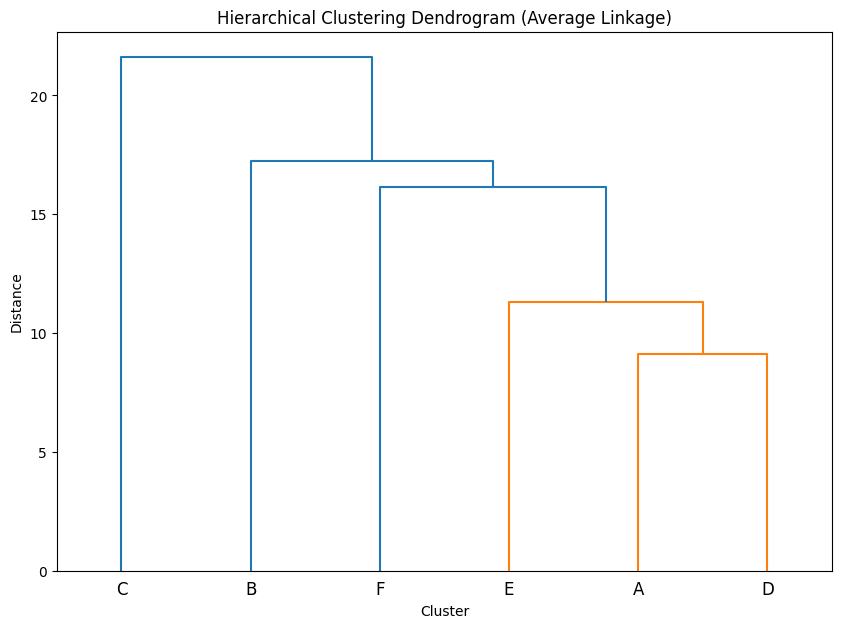
\includegraphics[width=0.8\textwidth]{dendrogram.png}
  \caption{Hierarchical Clustering Dendrogram (Average Linkage)}
  \label{fig:dendrogram}
\end{figure}


\problem{Logistic Regression and Regularization}

\subsection{Optimization Problem}
The logistic regression optimization problem with L2 regularization is given by:
\[
\min_{\bm{\beta}} \sum_{i=1}^{m} \left[ y_i \bm{\beta}^T \hat{\bm{x}}_i - \log{\left(1 + e^{\bm{\beta}^T \hat{\bm{x}}_i}\right)} \right] + \lambda \|\bm{\beta}\|^2_2
\]

\subsection{Gradient Derivation}
The gradient of the objective function with respect to \(\bm{\beta}\) is:
\[
\nabla_{\bm{\beta}} = \sum_{i=1}^{m} \left( y_i \hat{\bm{x}}_i - \frac{e^{\bm{\beta}^T \hat{\bm{x}}_i}}{1 + e^{\bm{\beta}^T \hat{\bm{x}}_i}} \hat{\bm{x}}_i \right) + 2 \lambda \bm{\beta}
\]
Simplifying the expression inside the sum:
\[
\nabla_{\bm{\beta}} = \sum_{i=1}^{m} \left( y_i - \sigma(\bm{\beta}^T \hat{\bm{x}}_i) \right) \hat{\bm{x}}_i + 2 \lambda \bm{\beta}
\]
where \(\sigma(z) = \frac{1}{1 + e^{-z}}\) is the sigmoid function.

\subsection{Parameter Update Formula}
Using gradient descent, the parameter update rule is:
\[
\bm{\beta} \leftarrow \bm{\beta} - \alpha \nabla_{\bm{\beta}}
\]
where \(\alpha\) is the learning rate. Substituting the gradient:
\[
\bm{\beta} \leftarrow \bm{\beta} - \alpha \left( \sum_{i=1}^{m} \left( y_i - \sigma(\bm{\beta}^T \hat{\bm{x}}_i) \right) \hat{\bm{x}}_i + 2 \lambda \bm{\beta} \right)
\]


\vspace{2mm}
\end{document}
